%**************************************************************************************
% License:
% CC BY-NC-SA 4.0 (http://creativecommons.org/licenses/by-nc-sa/4.0/)
%**************************************************************************************

\documentclass[aspectratio=169]{beamer}

\mode<presentation> {
	\usetheme{Madrid}
	
	% Burnt orange
	\definecolor{burntorange}{rgb}{0.8, 0.33, 0.0}
	\colorlet{beamer@blendedblue}{burntorange}
	% Pale yellow
	\definecolor{paleyellow}{rgb}{1.0, 1.0, 0.953}
	\setbeamercolor{background canvas}{bg=paleyellow}
	% Secondary and tertiary palette
	\setbeamercolor*{palette secondary}{use=structure,fg=white,bg=burntorange!80!black}
	\setbeamercolor*{palette tertiary}{use=structure,fg=white,bg=burntorange!60!black}
	
	% Remove navigation symbols
	\setbeamertemplate{navigation symbols}{}
}

\usepackage{amsmath,amssymb,amsthm}
\usepackage{bm}
\usepackage{booktabs}
\usepackage{graphicx}
\usepackage[labelsep=space,tableposition=top]{caption}
\renewcommand{\figurename}{Fig.} 
\usepackage{caption,subcaption}
\usepackage{xcolor}
\usepackage{transparent}
\usepackage{hyperref}
\usepackage{tikz}
\usepackage{listings}
\usepackage{algorithm}
\usepackage{algorithmic}

% Define math operators
\DeclareMathOperator*{\argmin}{arg\,min}
\DeclareMathOperator*{\argmax}{arg\,max}
\DeclareMathOperator{\ReLU}{ReLU}

% Code listing style
\lstset{
    language=Python,
    basicstyle=\tiny\ttfamily,
    keywordstyle=\color{blue},
    commentstyle=\color{gray},
    stringstyle=\color{green!70!black},
    showstringspaces=false,
    frame=single,
    breaklines=true,
    numbers=left,
    numberstyle=\tiny
}

%\AtBeginSection[]{
%	\begin{frame}{Outline}
%		\tableofcontents[currentsection, hideallsubsections]
%	\end{frame}
%}

%----------------------------------------------------------------------------------------
%	TITLE PAGE
%----------------------------------------------------------------------------------------
\title[Neural Networks \& Function Approximation]{Neural Networks and Function Approximation} 
\subtitle{Multi-Layer Perceptrons in Scientific Machine Learning}
\author{Krishna Kumar}
\institute[UT Austin]{
	University of Texas at Austin \\
	\medskip
	\textit{\url{krishnak@utexas.edu}}
}
\date{}

\begin{document}

\begin{frame}
\titlepage
\end{frame}

\begin{frame}{Outline}
\tableofcontents
\end{frame}

%----------------------------------------------------------------------------------------
% SECTION 1: Introduction and Motivation
%----------------------------------------------------------------------------------------
\section{Introduction and Motivation}

\begin{frame}{The Central Challenge}
\begin{block}{Core Question}
Can we build a machine that learns to approximate any continuous function from data?
\end{block}

\vspace{0.5cm}

\textbf{Applications in Scientific Machine Learning:}
\begin{itemize}
    \item Solving PDEs without mesh generation
    \item Learning constitutive models from experiments
    \item Surrogate modeling for expensive simulations
    \item System identification and control
    \item Inverse problems
\end{itemize}

\vspace{0.5cm}

\textbf{What we'll cover:}
\begin{itemize}
    \item Mathematical foundations (Weierstrass $\rightarrow$ UAT)
    \item Building blocks (perceptron $\rightarrow$ networks)
    \item Training algorithms (gradient descent, backpropagation)
    \item Automatic differentiation
    \item Practical implementation
\end{itemize}
\end{frame}

%----------------------------------------------------------------------------------------
% SECTION 2: The Benchmark Problem
%----------------------------------------------------------------------------------------
\section{The 1D Poisson Equation: Our Benchmark Problem}

\begin{frame}{Problem Formulation}
\begin{columns}
\column{0.5\textwidth}
\begin{block}{1D Poisson Equation}
\begin{align}
-\frac{d^2u}{dx^2} &= f(x), \quad x \in [0, 1]\\
u(0) &= 0, \quad u(1) = 0
\end{align}
\end{block}

\textbf{Physical interpretation:}
\begin{itemize}
    \item Heat conduction in a rod
    \item Deflection of a loaded beam
    \item Electrostatic potential
\end{itemize}

\column{0.5\textwidth}
For $f(x) = \pi^2 \sin(\pi x)$:
$$u(x) = \sin(\pi x)$$

\begin{figure}
    \centering
    \includegraphics[width=\textwidth]{figs/poisson-analytical-solution.png}
\end{figure}
\end{columns}
\end{frame}

\begin{frame}{The Function Approximation Challenge}
\begin{columns}
\column{0.5\textwidth}
\textbf{The Challenge:}
\begin{itemize}
    \item Given: 15 noisy measurements
    \item Goal: Reconstruct continuous $u(x)$
    \item Satisfy physics (PDE)
    \item Compute accurate derivatives
\end{itemize}

\vspace{0.5cm}
\textbf{Why is this hard?}
\begin{itemize}
    \item Sparse data
    \item Noise in measurements
    \item Need smooth interpolation
    \item Must satisfy constraints
\end{itemize}

\column{0.5\textwidth}
\begin{figure}
    \centering
    \includegraphics[width=\textwidth]{figs/sparse-data-challenge.png}
    \caption{Learning from sparse, noisy data}
\end{figure}
\end{columns}
\end{frame}

%----------------------------------------------------------------------------------------
% SECTION 3: Traditional Methods
%----------------------------------------------------------------------------------------
\section{Traditional Methods: Finite Difference}

\begin{frame}{Finite Difference Method}
\begin{columns}
\column{0.5\textwidth}
\textbf{Discretization:}
\begin{itemize}
    \item Grid points: $x_i = ih$
    \item Grid spacing: $h = 1/(n+1)$
    \item Unknown values: $u_i \approx u(x_i)$
\end{itemize}

\textbf{Derivative approximation:}
$$\frac{d^2u}{dx^2}\bigg|_{x_i} \approx \frac{u_{i+1} - 2u_i + u_{i-1}}{h^2}$$

\textbf{Linear system:}
$$\mathbf{A}\mathbf{u} = \mathbf{f}$$

\column{0.5\textwidth}
\begin{figure}
    \centering
    \includegraphics[width=\textwidth]{figs/finite-difference-methods.png}
\end{figure}
\end{columns}
\end{frame}

\begin{frame}{Finite Difference Solutions}
\begin{figure}
    \centering
    \includegraphics[width=0.8\textwidth]{figs/fd-poisson.png}
\end{figure}

\textbf{Key Limitations:}
\begin{itemize}
    \item Solution only at grid points
    \item Accuracy depends on grid resolution
    \item Not differentiable between points
    \item Curse of dimensionality in higher dimensions
\end{itemize}
\end{frame}

%----------------------------------------------------------------------------------------
% SECTION 4: From Polynomials to Neural Networks
%----------------------------------------------------------------------------------------
\section{From Polynomials to Neural Networks: The Weierstrass Path}

\begin{frame}{The Weierstrass Approximation Theorem (1885)}
\begin{block}{Theorem}
For any continuous function $f: [a,b] \to \mathbb{R}$ and any $\epsilon > 0$, there exists a polynomial $P$ such that:
$$\sup_{x \in [a,b]} |f(x) - P(x)| < \epsilon$$
\end{block}

\vspace{0.5cm}
\textbf{Key insight:} Simple building blocks (monomials) can approximate arbitrarily complex continuous functions.

\vspace{0.5cm}
\textbf{Historical progression:}
\begin{itemize}
    \item 1885: Weierstrass - Polynomials are universal
    \item 1937: Stone-Weierstrass - Generalization
    \item 1989: Cybenko - Neural networks are universal
    \item 1991: Hornik - General activation functions
\end{itemize}
\end{frame}

\begin{frame}{Why This Matters for Neural Networks}
\begin{columns}
\column{0.5\textwidth}
\textbf{Polynomials:}
\begin{itemize}
    \item Building blocks: $1, x, x^2, x^3, ...$
    \item Linear combination: $\sum a_n x^n$
    \item Global support
    \item Fixed basis
\end{itemize}

\vspace{0.5cm}
\textbf{Neural Networks:}
\begin{itemize}
    \item Building blocks: $\sigma(wx + b)$
    \item Linear combination: $\sum \alpha_i \sigma(w_i x + b_i)$
    \item Local support (ReLU)
    \item Adaptive basis
\end{itemize}

\column{0.5\textwidth}
\begin{figure}
    \centering
    \includegraphics[width=\textwidth]{figs/polynomial-approximation-sinpi.png}
    \caption{Polynomial approximation}
\end{figure}
\end{columns}
\end{frame}

\begin{frame}{Convergence Analysis}
\begin{columns}
\column{0.5\textwidth}
\textbf{Polynomial convergence:}
\begin{itemize}
    \item Degree 3: Error $\approx 0.05$
    \item Degree 5: Error $\approx 0.008$
    \item Degree 7: Error $\approx 0.001$
    \item Degree 9: Error $\approx 0.0001$
\end{itemize}

\textbf{Convergence rate:}
For $f \in C^k[0,1]$:
$$\|f - P_n\|_\infty = O(n^{-k})$$

\column{0.5\textwidth}
\begin{figure}
    \centering
    \includegraphics[width=\textwidth]{figs/polynomial-convergence.png}
    \caption{Exponential convergence for smooth functions}
\end{figure}
\end{columns}
\end{frame}

\begin{frame}{Bernstein Polynomials: Constructive Proof}
\begin{columns}
\column{0.5\textwidth}
\textbf{Bernstein basis:}
$$B_{k,n}(x) = \binom{n}{k} x^k (1-x)^{n-k}$$

\textbf{Approximation:}
$$B_n[f](x) = \sum_{k=0}^{n} f\left(\frac{k}{n}\right) B_{k,n}(x)$$

\textbf{Properties:}
\begin{itemize}
    \item Partition of unity
    \item Non-negative
    \item Uniform convergence
\end{itemize}

\column{0.5\textwidth}
\begin{figure}
    \centering
    \includegraphics[width=\textwidth]{figs/bernstein-approximation.png}
    \caption{Bernstein polynomial basis functions}
\end{figure}
\end{columns}
\end{frame}

\begin{frame}{Polynomial vs Neural Network Comparison}
\begin{figure}
    \centering
    \includegraphics[width=0.9\textwidth]{figs/polynomial-vs-nn-comparison.png}
\end{figure}

\textbf{Key differences:}
\begin{columns}
\column{0.5\textwidth}
\textbf{Polynomials:}
\begin{itemize}
    \item Global oscillations (Runge)
    \item Numerical instability
    \item Poor extrapolation
\end{itemize}

\column{0.5\textwidth}
\textbf{Neural Networks:}
\begin{itemize}
    \item Local adaptivity
    \item Numerical stability
    \item Better generalization
\end{itemize}
\end{columns}
\end{frame}

\begin{frame}{Limitations of Polynomial Approximation}
\begin{columns}
\column{0.5\textwidth}
\textbf{Runge's Phenomenon:}
\begin{itemize}
    \item Oscillations near boundaries
    \item Worse with equispaced points
    \item Amplified with degree
\end{itemize}

\textbf{Computational issues:}
\begin{itemize}
    \item Condition number $\sim 2^n$
    \item Global support
    \item No adaptivity
\end{itemize}

\column{0.5\textwidth}
\begin{figure}
    \centering
    \includegraphics[width=\textwidth]{figs/high-freq-comparison.png}
    \caption{High-frequency function challenges}
\end{figure}
\end{columns}
\end{frame}

\begin{frame}{From Weierstrass to Universal Approximation}
\begin{center}
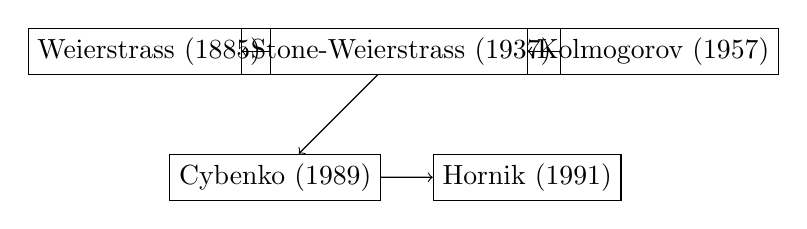
\begin{tikzpicture}[scale=0.8]
    \node[draw, rectangle] (w) at (0,0) {Weierstrass (1885)};
    \node[draw, rectangle] (s) at (4,0) {Stone-Weierstrass (1937)};
    \node[draw, rectangle] (k) at (8,0) {Kolmogorov (1957)};
    \node[draw, rectangle] (c) at (2,-2) {Cybenko (1989)};
    \node[draw, rectangle] (h) at (6,-2) {Hornik (1991)};
    
    \draw[->] (w) -- (s);
    \draw[->] (s) -- (k);
    \draw[->] (s) -- (c);
    \draw[->] (c) -- (h);
\end{tikzpicture}
\end{center}

\textbf{Evolution of approximation theory:}
\begin{itemize}
    \item Polynomials $\rightarrow$ General function algebras
    \item Single variable $\rightarrow$ Multiple variables
    \item Fixed basis $\rightarrow$ Adaptive basis
    \item Theoretical $\rightarrow$ Practical algorithms
\end{itemize}
\end{frame}

%----------------------------------------------------------------------------------------
% SECTION 5: The Neural Network Approach
%----------------------------------------------------------------------------------------
\section{The Neural Network Approach: Function Approximation}

\begin{frame}{Traditional vs Neural Network: Discrete vs Continuous}
\begin{columns}
\column{0.5\textwidth}
\textbf{Traditional (FD/FEM):}
\begin{itemize}
    \item Discretize domain
    \item Solve at grid points
    \item Interpolate between
    \item Result: Discrete values
\end{itemize}

$$u_h = \sum_{i} u_i \phi_i(x)$$

\column{0.5\textwidth}
\textbf{Neural Network:}
\begin{itemize}
    \item Continuous representation
    \item Defined everywhere
    \item Differentiable
    \item Result: Function
\end{itemize}

$$u_{NN}(x) = \sum_{i} \alpha_i \sigma(w_i x + b_i)$$
\end{columns}

\vspace{0.5cm}
\begin{block}{Key Advantage}
Neural networks provide a continuous, differentiable function that can be evaluated and differentiated anywhere in the domain.
\end{block}
\end{frame}

%----------------------------------------------------------------------------------------
% SECTION 6: The Perceptron
%----------------------------------------------------------------------------------------
\section{The Perceptron: Building Block of Neural Networks}

\begin{frame}{The Perceptron Model}
\begin{columns}
\column{0.5\textwidth}
\textbf{Mathematical model:}
$$y = \sigma(\mathbf{w}^T\mathbf{x} + b)$$

\textbf{Components:}
\begin{itemize}
    \item Input: $\mathbf{x} \in \mathbb{R}^n$
    \item Weights: $\mathbf{w} \in \mathbb{R}^n$
    \item Bias: $b \in \mathbb{R}$
    \item Activation: $\sigma(\cdot)$
    \item Output: $y \in \mathbb{R}$
\end{itemize}

\textbf{Geometric interpretation:}
Hyperplane $\mathbf{w}^T\mathbf{x} + b = 0$

\column{0.5\textwidth}
\begin{figure}
    \centering
    \includegraphics[width=\textwidth]{figs/perceptron.png}
\end{figure}
\end{columns}
\end{frame}

\begin{frame}[fragile]{Linear Perceptron in NumPy}
\begin{columns}
\column{0.55\textwidth}
\begin{lstlisting}
import numpy as np

class LinearPerceptron:
    def __init__(self, n_features):
        # Initialize weights randomly
        self.w = np.random.randn(n_features)
        self.b = np.random.randn()
    
    def forward(self, X):
        """Compute output"""
        return np.dot(X, self.w) + self.b
    
    def predict(self, X):
        """Make predictions"""
        return self.forward(X)

# Example usage
perceptron = LinearPerceptron(2)
X = np.array([[1, 2], [3, 4]])
y_pred = perceptron.predict(X)
print(f"Predictions: {y_pred}")
\end{lstlisting}

\column{0.45\textwidth}
\textbf{Pure linear model:}
$$\hat{y} = \mathbf{w}^T\mathbf{x} + b$$

\textbf{Limitations:}
\begin{itemize}
    \item Only linear boundaries
    \item Cannot learn XOR
    \item Limited expressiveness
\end{itemize}

\textbf{Solution:}
Add nonlinear activation!
\end{columns}
\end{frame}

\begin{frame}[fragile]{Training: Gradient Descent from Scratch}
\begin{lstlisting}
def train_perceptron(X, y, epochs=1000, lr=0.01):
    n_samples, n_features = X.shape
    w = np.random.randn(n_features)
    b = np.random.randn()
    
    for epoch in range(epochs):
        # Forward pass
        z = np.dot(X, w) + b
        y_pred = sigmoid(z)
        
        # Compute loss
        loss = 0.5 * np.mean((y - y_pred)**2)
        
        # Backward pass (compute gradients)
        error = y_pred - y
        dz = error * sigmoid_derivative(z)
        dw = np.dot(X.T, dz) / n_samples
        db = np.mean(dz)
        
        # Update parameters
        w -= lr * dw
        b -= lr * db
        
        if epoch % 100 == 0:
            print(f"Epoch {epoch}, Loss: {loss:.4f}")
    
    return w, b
\end{lstlisting}
\end{frame}

\begin{frame}{Gradient Computation Details}
\textbf{Loss function:}
$$L = \frac{1}{2}(y - \hat{y})^2$$

\textbf{Chain rule for gradient:}
$$\frac{\partial L}{\partial w_i} = \frac{\partial L}{\partial \hat{y}} \cdot \frac{\partial \hat{y}}{\partial z} \cdot \frac{\partial z}{\partial w_i}$$

\textbf{Component derivatives:}
\begin{align}
\frac{\partial L}{\partial \hat{y}} &= -(y - \hat{y}) \\
\frac{\partial \hat{y}}{\partial z} &= \sigma'(z) \\
\frac{\partial z}{\partial w_i} &= x_i
\end{align}

\textbf{Final gradient:}
$$\frac{\partial L}{\partial w_i} = -(y - \hat{y}) \cdot \sigma'(z) \cdot x_i$$
\end{frame}

\begin{frame}{Example: Linear Classification}
\begin{columns}
\column{0.5\textwidth}
\textbf{Linearly separable data:}
\begin{itemize}
    \item Two classes
    \item Can be separated by a line
    \item Perceptron converges
\end{itemize}

\textbf{Decision boundary:}
$$w_1 x_1 + w_2 x_2 + b = 0$$

\textbf{Classification rule:}
$$\text{class} = \begin{cases}
1 & \text{if } \sigma(z) > 0.5 \\
0 & \text{otherwise}
\end{cases}$$

\column{0.5\textwidth}
\begin{figure}
    \centering
    \includegraphics[width=\textwidth]{figs/linear-network-failure.png}
\end{figure}
\end{columns}
\end{frame}

\begin{frame}{Limitation: The XOR Problem}
\begin{columns}
\column{0.5\textwidth}
\textbf{XOR Truth Table:}
\begin{center}
\begin{tabular}{cc|c}
$x_1$ & $x_2$ & XOR \\
\hline
0 & 0 & 0 \\
0 & 1 & 1 \\
1 & 0 & 1 \\
1 & 1 & 0 \\
\end{tabular}
\end{center}

\textbf{The problem:}
\begin{itemize}
    \item Not linearly separable
    \item No single line works
    \item Perceptron fails
\end{itemize}

\column{0.5\textwidth}
\begin{figure}
    \centering
    \includegraphics[width=\textwidth]{figs/xor-problem.png}
\end{figure}
\end{columns}
\end{frame}

\begin{frame}{Mathematical Proof: XOR Impossibility}
\textbf{Assume linear separator exists:} $w_1 x_1 + w_2 x_2 + b = 0$

\textbf{Requirements from XOR:}
\begin{align}
(0,0): & \quad b < 0 \quad \text{(class 0)} \\
(0,1): & \quad w_2 + b > 0 \quad \text{(class 1)} \\
(1,0): & \quad w_1 + b > 0 \quad \text{(class 1)} \\
(1,1): & \quad w_1 + w_2 + b < 0 \quad \text{(class 0)}
\end{align}

\textbf{Contradiction:}
\begin{itemize}
    \item From (1): $b < 0$
    \item From (2) and (3): $w_1, w_2 > -b > 0$
    \item Adding (2) and (3): $w_1 + w_2 + 2b > 0$
    \item But (4) requires: $w_1 + w_2 + b < 0$
    \item Subtracting: $b > 0$ contradicts $b < 0$
\end{itemize}

$\Rightarrow$ No linear solution exists!
\end{frame}

\begin{frame}[fragile]{Solution: Adding Nonlinear Activation}
\begin{columns}
\column{0.55\textwidth}
\begin{lstlisting}
class NonlinearPerceptron:
    def __init__(self, n_features):
        self.w = np.random.randn(n_features)
        self.b = np.random.randn()
    
    def sigmoid(self, z):
        return 1 / (1 + np.exp(-z))
    
    def sigmoid_derivative(self, z):
        s = self.sigmoid(z)
        return s * (1 - s)
    
    def forward(self, X):
        z = np.dot(X, self.w) + self.b
        return self.sigmoid(z)
    
    def compute_gradients(self, X, y):
        z = np.dot(X, self.w) + self.b
        y_pred = self.sigmoid(z)
        
        error = y_pred - y
        dz = error * self.sigmoid_derivative(z)
        dw = np.dot(X.T, dz) / len(X)
        db = np.mean(dz)
        
        return dw, db
\end{lstlisting}

\column{0.45\textwidth}
\textbf{Key addition:}
Sigmoid activation
$$\sigma(z) = \frac{1}{1 + e^{-z}}$$

\textbf{Properties:}
\begin{itemize}
    \item Smooth, differentiable
    \item Bounded: $(0, 1)$
    \item Gradient: $\sigma'(z) = \sigma(z)(1-\sigma(z))$
\end{itemize}

But still can't solve XOR with single neuron!
\end{columns}
\end{frame}

%----------------------------------------------------------------------------------------
% SECTION 7: Backpropagation
%----------------------------------------------------------------------------------------
\section{Backpropagation with Activation Functions}

\begin{frame}{Backpropagation Algorithm}
\begin{columns}
\column{0.5\textwidth}
\textbf{Forward Pass:}
\begin{enumerate}
    \item Compute activations layer by layer
    \item Store intermediate values
    \item Calculate loss
\end{enumerate}

\textbf{Backward Pass:}
\begin{enumerate}
    \item Start from output error
    \item Propagate error backward
    \item Compute gradients via chain rule
    \item Update weights
\end{enumerate}

\column{0.5\textwidth}
\begin{algorithmic}
\STATE \textbf{Forward:}
\FOR{layer $l = 1$ to $L$}
    \STATE $z^{(l)} = W^{(l)}a^{(l-1)} + b^{(l)}$
    \STATE $a^{(l)} = \sigma(z^{(l)})$
\ENDFOR
\STATE
\STATE \textbf{Backward:}
\STATE $\delta^{(L)} = \nabla_a L \odot \sigma'(z^{(L)})$
\FOR{layer $l = L-1$ to $1$}
    \STATE $\delta^{(l)} = (W^{(l+1)})^T\delta^{(l+1)} \odot \sigma'(z^{(l)})$
\ENDFOR
\end{algorithmic}
\end{columns}
\end{frame}

\begin{frame}[fragile]{Backpropagation Implementation}
\begin{lstlisting}
def backpropagation(network, X, y):
    # Forward pass
    activations = [X]
    z_values = []
    
    for layer in network.layers:
        z = np.dot(activations[-1], layer.W) + layer.b
        z_values.append(z)
        a = layer.activation(z)
        activations.append(a)
    
    # Compute loss
    loss = 0.5 * np.mean((activations[-1] - y)**2)
    
    # Backward pass
    delta = (activations[-1] - y) * layer.activation_derivative(z_values[-1])
    gradients = []
    
    for i in reversed(range(len(network.layers))):
        # Gradient w.r.t weights and bias
        grad_W = np.dot(activations[i].T, delta) / len(X)
        grad_b = np.mean(delta, axis=0)
        gradients.append((grad_W, grad_b))
        
        # Propagate error backward
        if i > 0:
            delta = np.dot(delta, network.layers[i].W.T)
            delta *= network.layers[i-1].activation_derivative(z_values[i-1])
    
    return loss, list(reversed(gradients))
\end{lstlisting}
\end{frame}

%----------------------------------------------------------------------------------------
% SECTION 8: The Critical Role of Nonlinearity
%----------------------------------------------------------------------------------------
\section{The Role of Nonlinearity}

\begin{frame}{Why Nonlinearity is Essential}
\begin{columns}
\column{0.5\textwidth}
\textbf{Without activation:}
\begin{align}
h^{(2)} &= W^{(2)}h^{(1)} + b^{(2)} \\
&= W^{(2)}(W^{(1)}x + b^{(1)}) + b^{(2)} \\
&= W^{(2)}W^{(1)}x + W^{(2)}b^{(1)} + b^{(2)} \\
&= W_{eff}x + b_{eff}
\end{align}

Still linear! Multiple layers collapse.

\column{0.5\textwidth}
\textbf{With activation:}
$$h^{(2)} = \sigma(W^{(2)}\sigma(W^{(1)}x + b^{(1)}) + b^{(2)})$$

Truly nonlinear transformation!

\begin{figure}
    \centering
    \includegraphics[width=\textwidth]{figs/why-activation.png}
\end{figure}
\end{columns}
\end{frame}

\begin{frame}{Activation Functions Enable Complex Boundaries}
\begin{figure}
    \centering
    \includegraphics[width=0.9\textwidth]{figs/xor-decision-boundaries.png}
\end{figure}

\textbf{Key insight:} Nonlinear activations allow networks to:
\begin{itemize}
    \item Create curved decision boundaries
    \item Learn complex patterns
    \item Compose simple functions into complex ones
    \item Approximate any continuous function (UAT)
\end{itemize}
\end{frame}

%----------------------------------------------------------------------------------------
\begin{frame}{Common Activation Functions}
\begin{figure}
    \centering
    \includegraphics[width=0.9\textwidth]{figs/activation-functions.png}
\end{figure}

\begin{center}
\small
\begin{tabular}{lll}
\toprule
Function & Formula & Properties \\
\midrule
Sigmoid & $\sigma(x) = \frac{1}{1 + e^{-x}}$ & Smooth, $(0,1)$, vanishing gradient \\
Tanh & $\tanh(x) = \frac{e^x - e^{-x}}{e^x + e^{-x}}$ & Zero-centered, $(-1,1)$ \\
ReLU & $\max(0, x)$ & Simple, efficient, no saturation \\
Leaky ReLU & $\max(0.01x, x)$ & Avoids dead neurons \\
\bottomrule
\end{tabular}
\end{center}
\end{frame}

\begin{frame}{Activation Function Properties}
\begin{columns}
\column{0.5\textwidth}
\textbf{Sigmoid:}
\begin{itemize}
    \item Range: $(0, 1)$
    \item Derivative: $\sigma'(x) = \sigma(x)(1-\sigma(x))$
    \item Max gradient: 0.25
    \item Issue: Vanishing gradient
\end{itemize}

\textbf{Tanh:}
\begin{itemize}
    \item Range: $(-1, 1)$
    \item Derivative: $\tanh'(x) = 1 - \tanh^2(x)$
    \item Max gradient: 1
    \item Better than sigmoid
\end{itemize}

\column{0.5\textwidth}
\textbf{ReLU:}
\begin{itemize}
    \item Range: $[0, \infty)$
    \item Derivative: $\begin{cases} 1 & x > 0 \\ 0 & x \leq 0 \end{cases}$
    \item No vanishing gradient
    \item Issue: Dead neurons
\end{itemize}

\textbf{Modern variants:}
\begin{itemize}
    \item Swish: $x \cdot \sigma(x)$
    \item GELU: Gaussian Error Linear Unit
    \item Mish: $x \cdot \tanh(\ln(1+e^x))$
\end{itemize}
\end{columns}
\end{frame}

%----------------------------------------------------------------------------------------
% SECTION 10: Building Capacity
%----------------------------------------------------------------------------------------
\section{Building Capacity: Single Hidden Layer Networks}

\begin{frame}{Single Hidden Layer Architecture}
\begin{columns}
\column{0.5\textwidth}
\textbf{Network structure:}
\begin{align}
z^{(1)} &= W^{(1)}x + b^{(1)} \\
h &= \sigma(z^{(1)}) \\
z^{(2)} &= W^{(2)}h + b^{(2)} \\
y &= z^{(2)}
\end{align}

\textbf{Parameters:}
\begin{itemize}
    \item $W^{(1)} \in \mathbb{R}^{h \times n}$
    \item $b^{(1)} \in \mathbb{R}^h$
    \item $W^{(2)} \in \mathbb{R}^{1 \times h}$
    \item $b^{(2)} \in \mathbb{R}$
\end{itemize}

Total: $h(n+1) + (h+1)$

\column{0.5\textwidth}
\begin{figure}
    \centering
    \includegraphics[width=\textwidth]{figs/single-layer-nn1.png}
\end{figure}
\end{columns}
\end{frame}

\begin{frame}{Solving XOR with Hidden Layer}
\begin{columns}
\column{0.5\textwidth}
\textbf{Network solution:}
Hidden layer learns:
\begin{itemize}
    \item $h_1$: OR gate
    \item $h_2$: NAND gate
\end{itemize}

Output combines:
$$y = h_1 \land h_2 = \text{XOR}$$

\textbf{Weights example:}
\begin{itemize}
    \item $W^{(1)} = \begin{bmatrix} 20 & 20 \\ -20 & -20 \end{bmatrix}$
    \item $b^{(1)} = \begin{bmatrix} -10 \\ 30 \end{bmatrix}$
    \item $W^{(2)} = \begin{bmatrix} 20 & 20 \end{bmatrix}$
    \item $b^{(2)} = -30$
\end{itemize}

\column{0.5\textwidth}
\begin{figure}
    \centering
    \includegraphics[width=\textwidth]{figs/xor-decision-boundaries.png}
\end{figure}
\end{columns}
\end{frame}

\begin{frame}{Multiple Output Neurons}
\begin{columns}
\column{0.5\textwidth}
\textbf{Multi-class classification:}
\begin{itemize}
    \item Output layer: $m$ neurons
    \item Each neuron: one class
    \item Softmax activation:
\end{itemize}
$$p_i = \frac{e^{z_i}}{\sum_j e^{z_j}}$$

\textbf{Applications:}
\begin{itemize}
    \item Classification (MNIST)
    \item Multi-output regression
    \item Structured prediction
\end{itemize}

\column{0.5\textwidth}
\begin{figure}
    \centering
    \includegraphics[width=\textwidth]{figs/multioutput-perceptrons.png}
\end{figure}
\end{columns}
\end{frame}

%----------------------------------------------------------------------------------------
% SECTION 11: Training Neural Networks
%----------------------------------------------------------------------------------------
\section{Training Neural Networks}

\begin{frame}{The Training Process}
\begin{columns}
\column{0.5\textwidth}
\textbf{Optimization loop:}
\begin{enumerate}
    \item Initialize weights randomly
    \item Forward pass: compute predictions
    \item Compute loss
    \item Backward pass: compute gradients
    \item Update weights
    \item Repeat until convergence
\end{enumerate}

\textbf{Key components:}
\begin{itemize}
    \item Loss function
    \item Optimizer
    \item Learning rate
    \item Batch size
\end{itemize}

\column{0.5\textwidth}
\begin{figure}
    \centering
    \includegraphics[width=\textwidth]{figs/training-convergence.png}
\end{figure}
\end{columns}
\end{frame}

\begin{frame}{Loss Functions}
\textbf{Regression:}
\begin{itemize}
    \item MSE: $L = \frac{1}{N}\sum_{i=1}^N (y_i - \hat{y}_i)^2$
    \item MAE: $L = \frac{1}{N}\sum_{i=1}^N |y_i - \hat{y}_i|$
    \item Huber: Robust to outliers
\end{itemize}

\textbf{Classification:}
\begin{itemize}
    \item Cross-entropy: $L = -\sum_i y_i \log(\hat{y}_i)$
    \item Hinge loss: SVM-style
\end{itemize}

\end{frame}

%----------------------------------------------------------------------------------------
% SECTION 12: Automatic Differentiation
%----------------------------------------------------------------------------------------
\section{Computing Gradients with Automatic Differentiation}

\begin{frame}{The Core Insight: Functions are Computations}
\begin{columns}
\column{0.5\textwidth}
\textbf{Three approaches:}
\begin{enumerate}
    \item \textbf{Symbolic:} Manipulate expressions
    \item \textbf{Numerical:} Finite differences
    \item \textbf{Automatic:} Apply chain rule
\end{enumerate}

\textbf{Why AD wins:}
\begin{itemize}
    \item Exact to machine precision
    \item Efficient (linear cost)
    \item Handles any computation
\end{itemize}

\column{0.5\textwidth}
\begin{center}
\begin{tabular}{lll}
\toprule
Method & Accuracy & Speed \\
\midrule
Symbolic & Exact & Slow \\
Numerical & $O(h)$ & Fast \\
Automatic & Machine $\epsilon$ & Fast \\
\bottomrule
\end{tabular}
\end{center}

\vspace{0.5cm}
\textbf{Numerical issues:}
$$f'(x) \approx \frac{f(x+h) - f(x)}{h}$$
\begin{itemize}
    \item Truncation: $O(h)$
    \item Roundoff: $O(\epsilon/h)$
    \item Optimal: $h \sim \sqrt{\epsilon}$
\end{itemize}
\end{columns}
\end{frame}

\begin{frame}{Computational Graph}
\begin{columns}
\column{0.3\textwidth}
\textbf{Example:} $y = (x_1 + x_2) \cdot x_2$

\textbf{Forward computation:}
\begin{enumerate}
    \item $v_1 = x_1 = 2$
    \item $v_2 = x_2 = 3$
    \item $v_3 = v_1 + v_2 = 5$
    \item $v_4 = v_3 \cdot v_2 = 15$
\end{enumerate}

\textbf{Graph representation:}
Every operation becomes a node

\column{0.7\textwidth}
\begin{figure}
    \centering
    \includegraphics[width=\textwidth]{figs/ad1.png}
\end{figure}
\end{columns}
\end{frame}

%----------------------------------------------------------------------------------------
\begin{frame}{Forward Mode: Dual Numbers}
\begin{columns}
\column{0.5\textwidth}
\textbf{Dual number arithmetic:}
$$x = a + b\epsilon, \quad \epsilon^2 = 0$$

\textbf{Operations:}
\begin{align}
(a + b\epsilon) + (c + d\epsilon) &= (a+c) + (b+d)\epsilon \\
(a + b\epsilon) \times (c + d\epsilon) &= ac + (ad+bc)\epsilon \\
\sin(a + b\epsilon) &= \sin(a) + b\cos(a)\epsilon
\end{align}

\column{0.5\textwidth}
\textbf{Example:} $f(x) = x^2 + \sin(x)$ at $x=2$

Start: $x = 2 + 1\cdot\epsilon$
\begin{align}
x^2 &= 4 + 4\epsilon \\
\sin(x) &= \sin(2) + \cos(2)\epsilon \\
f(x) &= (4+\sin(2)) + (4+\cos(2))\epsilon
\end{align}

Result: $f(2)$ and $f'(2)$ simultaneously!
\end{columns}
\end{frame}

\begin{frame}{Forward Mode: Computing $\partial y/\partial x_1$}
\begin{figure}
    \centering
    \includegraphics[width=0.8\textwidth]{figs/ad3.png}
\end{figure}

Forward mode propagates derivatives alongside values from inputs to output.
\end{frame}

\begin{frame}{Forward Mode: Multiple Inputs}
\textbf{For $n$ inputs, need $n$ forward passes:}
\begin{itemize}
    \item Pass 1: Seed $(1, 0, 0, ...)$ for $\partial f/\partial x_1$
    \item Pass 2: Seed $(0, 1, 0, ...)$ for $\partial f/\partial x_2$
    \item ...
    \item Pass n: Seed $(0, 0, ..., 1)$ for $\partial f/\partial x_n$
\end{itemize}

\textbf{Computational cost:} $O(n \times \text{ops})$

\textbf{Best for:}
\begin{itemize}
    \item Few inputs, many outputs
    \item Computing Jacobian-vector products
    \item Sensitivity analysis
\end{itemize}
\end{frame}

%----------------------------------------------------------------------------------------
\begin{frame}{Reverse Mode: The Backward Pass}
\begin{columns}
\column{0.4\textwidth}
\textbf{Key idea:}
\begin{itemize}
    \item Forward: Compute values
    \item Backward: Compute gradients
    \item Use chain rule recursively
\end{itemize}

\textbf{Adjoint notation:}
$$\bar{v}_i = \frac{\partial y}{\partial v_i}$$

\textbf{Chain rule:}
$$\bar{v}_i = \sum_{j \in \text{children}(i)} \bar{v}_j \frac{\partial v_j}{\partial v_i}$$

\column{0.6\textwidth}
\begin{figure}
    \centering
    \includegraphics[width=\textwidth]{figs/ad7.png}
\end{figure}
\end{columns}
\end{frame}

\begin{frame}{Reverse Mode: Complete Example}
\textbf{Function:} $y = x_1^2 + x_2$

\begin{columns}
\column{0.5\textwidth}
\textbf{Forward pass:}
\begin{enumerate}
    \item $v_1 = x_1 = 2$
    \item $v_2 = x_2 = 3$
    \item $v_3 = v_1^2 = 4$
    \item $v_4 = v_3 + v_2 = 7$
\end{enumerate}

\column{0.5\textwidth}
\textbf{Backward pass:}
\begin{enumerate}
    \item $\bar{v}_4 = 1$ (seed)
    \item $\bar{v}_3 = \bar{v}_4 \cdot 1 = 1$
    \item $\bar{v}_2 = \bar{v}_4 \cdot 1 = 1$
    \item $\bar{v}_1 = \bar{v}_3 \cdot 2v_1 = 4$
\end{enumerate}
\end{columns}

\vspace{0.5cm}
\textbf{Result:} $\nabla y = (4, 1)$ in ONE backward pass!

\textbf{Cost:} $O(\text{ops})$ for all gradients
\end{frame}

\begin{frame}{Forward vs Reverse Mode}
\begin{center}
\begin{tabular}{lll}
\toprule
Aspect & Forward Mode & Reverse Mode \\
\midrule
Direction & Input $\rightarrow$ Output & Output $\rightarrow$ Input \\
Computes & Jacobian-vector product & Vector-Jacobian product \\
Cost for $f: \mathbb{R}^n \to \mathbb{R}^m$ & $O(n \times \text{ops})$ & $O(m \times \text{ops})$ \\
Best when & $n \ll m$ & $n \gg m$ \\
Memory & Low & High (store graph) \\
\bottomrule
\end{tabular}
\end{center}

\vspace{0.5cm}
\textbf{Machine Learning context:}
\begin{itemize}
    \item Millions of parameters (inputs)
    \item One loss function (output)
    \item $n \gg m = 1$
    \item \textbf{Reverse mode (backprop) wins!}
\end{itemize}
\end{frame}

\begin{frame}[fragile]{AD in PyTorch}
\begin{columns}
\column{0.55\textwidth}
\begin{lstlisting}
import torch

# Simple example
x = torch.tensor(2.0, requires_grad=True)
y = x**2 + torch.sin(x)
y.backward()
print(f"dy/dx = {x.grad}")
# Output: dy/dx = 4.0 + cos(2)

# Neural network example
class Net(torch.nn.Module):
    def __init__(self):
        super().__init__()
        self.fc1 = torch.nn.Linear(10, 50)
        self.fc2 = torch.nn.Linear(50, 1)
    
    def forward(self, x):
        x = torch.relu(self.fc1(x))
        return self.fc2(x)

model = Net()
x = torch.randn(32, 10)
y = model(x)
loss = y.mean()
loss.backward()  # Computes all gradients!
\end{lstlisting}

\column{0.45\textwidth}
\textbf{PyTorch autograd:}
\begin{itemize}
    \item Dynamic graph
    \item Automatic tracking
    \item Efficient backprop
\end{itemize}

\textbf{Key features:}
\begin{itemize}
    \item \texttt{requires\_grad=True}
    \item \texttt{backward()} method
    \item Gradient accumulation
    \item Graph optimization
\end{itemize}
\end{columns}
\end{frame}

%----------------------------------------------------------------------------------------
\section{Gradient Descent Optimization}

\begin{frame}{Gradient Descent Algorithm}
\begin{columns}
\column{0.35\textwidth}
\textbf{Basic algorithm:}
\begin{algorithmic}
\STATE Initialize $\theta_0$
\WHILE{not converged}
    \STATE $g_t = \nabla L(\theta_{t-1})$
    \STATE $\theta_t = \theta_{t-1} - \alpha g_t$
\ENDWHILE
\end{algorithmic}

\textbf{Variants:}
\begin{itemize}
    \item SGD: Single sample
    \item Mini-batch: Small subset
    \item Full batch: All data
\end{itemize}

\column{0.65\textwidth}
\begin{figure}
    \centering
    \includegraphics[width=\textwidth]{figs/sgd.png}
\end{figure}
\end{columns}
\end{frame}

\begin{frame}{Learning Rate Effects}
\begin{columns}
\column{0.35\textwidth}
\textbf{Too small ($\alpha = 0.001$):}
\begin{itemize}
    \item Slow convergence
    \item May get stuck
    \item Many iterations needed
\end{itemize}

\textbf{Too large ($\alpha = 1.0$):}
\begin{itemize}
    \item Oscillations
    \item May diverge
    \item Miss minimum
\end{itemize}

\textbf{Just right ($\alpha = 0.01$):}
\begin{itemize}
    \item Steady progress
    \item Reaches minimum
    \item Efficient convergence
\end{itemize}

\column{0.65\textwidth}
\begin{figure}
    \centering
    \includegraphics[width=\textwidth]{figs/training-validation-fit.png}
\end{figure}
\end{columns}
\end{frame}

\begin{frame}{Modern Optimizers}
\begin{columns}
\column{0.5\textwidth}
\textbf{Momentum SGD:}
$$v_t = \beta v_{t-1} + \nabla L(\theta_{t-1})$$
$$\theta_t = \theta_{t-1} - \alpha v_t$$

\textbf{Adam:}
\begin{itemize}
    \item Adaptive learning rates
    \item Momentum + RMSprop
    \item Bias correction
\end{itemize}

\column{0.5\textwidth}
\textbf{Comparison:}
\begin{center}
\small
\begin{tabular}{ll}
\toprule
Optimizer & Properties \\
\midrule
SGD & Simple, proven \\
Momentum & Accelerates \\
AdaGrad & Adaptive \\
RMSprop & Adaptive + stable \\
Adam & Best default \\
\bottomrule
\end{tabular}
\end{center}
\end{columns}
\end{frame}

%----------------------------------------------------------------------------------------
\section{Universal Approximation Theorem}

\begin{frame}{The Universal Approximation Theorem}
\begin{block}{Theorem (Cybenko 1989, Hornik 1991)}
Let $\sigma$ be a continuous, non-polynomial activation function. For any continuous function $f: [0,1]^n \to \mathbb{R}$ and any $\epsilon > 0$, there exists a single-hidden-layer network:
$$N(x) = \sum_{i=1}^m \alpha_i \sigma(\mathbf{w}_i^T\mathbf{x} + b_i)$$
such that $\sup_{x \in [0,1]^n} |f(x) - N(x)| < \epsilon$
\end{block}

\textbf{Key points:}
\begin{itemize}
    \item One hidden layer suffices
    \item Width determines accuracy
    \item Says nothing about learnability
    \item Continuity is essential
\end{itemize}
\end{frame}

\begin{frame}{What the Theorem States}
\textbf{Formally:} Neural networks are dense in $C([0,1]^n)$

\textbf{Intuitively:}
\begin{itemize}
    \item Any continuous function can be approximated
    \item To any desired accuracy
    \item With enough neurons
\end{itemize}

\textbf{What it doesn't say:}
\begin{itemize}
    \item How many neurons needed
    \item How to find the weights
    \item Whether deep is better than wide
    \item Generalization guarantees
\end{itemize}

\textbf{Practical implications:}
\begin{itemize}
    \item Neural networks are universal function approximators
    \item Theoretical foundation for deep learning
    \item Justifies use in scientific computing
\end{itemize}
\end{frame}

\begin{frame}{Why This Matters for SciML}
\textbf{Traditional numerical methods:}
\begin{itemize}
    \item Fixed basis functions (polynomials, Fourier)
    \item Problem-specific methods
    \item Mesh-based discretization
\end{itemize}

\textbf{Neural networks (UAT guarantee):}
\begin{itemize}
    \item Adaptive basis functions
    \item Universal approximation capability
    \item Mesh-free representation
    \item Differentiable everywhere
\end{itemize}

\textbf{Applications enabled:}
\begin{itemize}
    \item Physics-informed neural networks (PINNs)
    \item Neural ODEs/PDEs
    \item Operator learning
    \item Inverse problems
\end{itemize}
\end{frame}

%----------------------------------------------------------------------------------------
\section{Mathematical Foundations: Function Spaces}

\begin{frame}{Banach Spaces: The Setting}
\begin{block}{Definition}
A Banach space is a complete normed vector space.
\end{block}

\textbf{For function approximation:}
\begin{itemize}
    \item $C([a,b])$: Continuous functions
    \item Norm: $\|f\|_\infty = \sup_{x \in [a,b]} |f(x)|$
    \item Complete: Cauchy sequences converge
\end{itemize}

\textbf{Key property - Density:}
\begin{block}{Dense Subset}
$S \subseteq X$ is dense if for every $f \in X$ and $\epsilon > 0$, there exists $g \in S$ with $\|f - g\| < \epsilon$
\end{block}

UAT says: Neural networks are dense in $C([0,1]^n)$
\end{frame}

\begin{frame}{Hilbert Spaces: Adding Geometry}
\textbf{Inner product space:}
$$\langle f, g \rangle = \int_a^b f(x)g(x) dx$$

\textbf{Induced norm:}
$$\|f\|_2 = \sqrt{\langle f, f \rangle}$$

\textbf{Orthogonal basis:}
\begin{itemize}
    \item Fourier: $\{\sin(n\pi x), \cos(n\pi x)\}$
    \item Legendre polynomials
    \item Wavelets
\end{itemize}

\textbf{Neural networks vs orthogonal basis:}
\begin{itemize}
    \item Adaptive vs fixed
    \item Local vs global
    \item Nonlinear vs linear combination
\end{itemize}
\end{frame}

%----------------------------------------------------------------------------------------

\begin{frame}{Constructive Proof with ReLU}
\textbf{Key idea:} Build piecewise linear approximations

\textbf{ReLU building blocks:}
$$\text{bump}_{[a,b]}(x) = \ReLU(x-a) - \ReLU(x-b)$$

\begin{columns}
\column{0.5\textwidth}
\textbf{Algorithm:}
\begin{enumerate}
    \item Divide $[0,1]$ into intervals
    \item Approximate linearly on each
    \item Use ReLUs to create pieces
    \item Sum to get approximation
\end{enumerate}

\column{0.5\textwidth}
\begin{figure}
    \centering
    \includegraphics[width=0.7\textwidth]{figs/relu-decomposition-sinpi.png}
\end{figure}
\end{columns}
\end{frame}

\begin{frame}{Building Blocks: The Role of Bias}
\begin{columns}
\column{0.35\textwidth}
\textbf{Single ReLU:}
$$h = \ReLU(wx + b)$$

\textbf{Breakpoint location:}
$$wx + b = 0 \Rightarrow x = -b/w$$

\textbf{Bias controls position!}

\column{0.65\textwidth}
\begin{figure}
    \centering
    \includegraphics[width=\textwidth]{figs/bias-breakpoints-detailed.png}
\end{figure}
\end{columns}

\textbf{Creating complex functions:}
Combine multiple ReLUs with different biases to approximate any continuous function
\end{frame}

\begin{frame}{Proof by Contradiction (Hahn-Banach)}
\textbf{Assume:} Neural networks NOT dense in $C([0,1])$

\textbf{Then:} Exists $f^*$ and $\epsilon > 0$ such that
$$\|f^* - g\|_\infty \geq \epsilon \quad \forall g \in \mathcal{N}$$

\textbf{By Hahn-Banach:} Exists linear functional $L$ with
\begin{itemize}
    \item $L(f^*) \neq 0$
    \item $L(g) = 0$ for all neural networks $g$
\end{itemize}

\textbf{By Riesz:} $L$ corresponds to measure $\mu$
$$L(f) = \int f d\mu$$

\textbf{Contradiction:} $\mu$ must annihilate all half-spaces $\Rightarrow$ $\mu = 0$ $\Rightarrow$ $L(f^*) = 0$
\end{frame}

\begin{frame}{Visualization of the Contradiction}
\begin{figure}
    \centering
    \includegraphics[width=0.6\textwidth]{figs/contradiction-visualization.png}
\end{figure}

If neural networks can't approximate some continuous function, a "detector" measure must exist. But this detector must be zero everywhere—contradiction!
\end{frame}

%----------------------------------------------------------------------------------------
\section{What Neural Networks Cannot Approximate}

\begin{frame}{The Continuity Requirement}
\textbf{Key limitation:} Neural networks with continuous activations can only approximate continuous functions

\textbf{Example - Step function:}
$$H(x) = \begin{cases} 0 & x < 0.5 \\ 1 & x \geq 0.5 \end{cases}$$

\textbf{Why it fails:}
\begin{itemize}
    \item Continuous functions cannot have jumps
    \item Sigmoid approximation always smooth
    \item Error at discontinuity never vanishes
\end{itemize}

\textbf{Different norms:}
\begin{itemize}
    \item $L^\infty$: Poor (max error at jump)
    \item $L^2$: Good (integral of error small)
    \item $L^1$: Good (average error small)
\end{itemize}
\end{frame}

\begin{frame}{The Detector That Distinguishes}
\textbf{Signed measure detector:}
$$\mu = +1 \text{ on } [0, 0.5), \quad -1 \text{ on } [0.5, 1]$$

\textbf{Applied to different functions:}
\begin{itemize}
    \item Step function: $\int H d\mu = -0.5$
    \item Continuous approximation: $\int f d\mu \approx 0$
    \item Neural network: Always $\approx 0$
\end{itemize}

\textbf{This detector reveals:}
Neural networks cannot perfectly approximate discontinuous functions in supremum norm

\textbf{Practical implications:}
\begin{itemize}
    \item Shocks in PDEs need special treatment
    \item Material interfaces challenging
    \item Use domain decomposition
\end{itemize}
\end{frame}

%----------------------------------------------------------------------------------------
\section{Practical Implementation}

\begin{frame}{Width vs Approximation Quality}
\begin{columns}
\column{0.5\textwidth}
\textbf{Experimental setup:}
\begin{itemize}
    \item Target: $\sin(\pi x)$
    \item Networks: 5, 10, 20, 50 neurons
    \item Training: 1000 epochs
    \item Optimizer: Adam
\end{itemize}

\textbf{Results:}
\begin{itemize}
    \item 5 neurons: Error $\sim 10^{-2}$
    \item 10 neurons: Error $\sim 10^{-3}$
    \item 20 neurons: Error $\sim 10^{-4}$
    \item 50 neurons: Error $\sim 10^{-5}$
\end{itemize}

\column{0.5\textwidth}
\begin{figure}
    \centering
    \includegraphics[width=\textwidth]{figs/width-quality.png}
\end{figure}
\end{columns}
\end{frame}

\begin{frame}{Width vs Error: Quantitative Analysis}
\begin{figure}
    \centering
    \includegraphics[width=0.8\textwidth]{figs/width-vs-error.png}
\end{figure}

\textbf{Key observations:}
\begin{itemize}
    \item Power law: Error $\sim N^{-\alpha}$
    \item Diminishing returns
    \item Optimization challenges for very wide networks
\end{itemize}
\end{frame}

\begin{frame}{Training and Validation}
\begin{figure}
    \centering
    \includegraphics[width=0.8\textwidth]{figs/training-validation-fit.png}
\end{figure}

\textbf{Detecting overfitting:}
\begin{itemize}
    \item Training loss decreases
    \item Validation loss increases
    \item Gap indicates overfitting
    \item Use early stopping
\end{itemize}
\end{frame}

\begin{frame}{Overfitting and Regularization}
\begin{columns}
\column{0.35\textwidth}
\textbf{Overfitting symptoms:}
\begin{itemize}
    \item Perfect training fit
    \item Poor generalization
    \item High-frequency oscillations
\end{itemize}

\textbf{Regularization techniques:}
\begin{itemize}
    \item $L_2$ penalty: $\lambda \|W\|^2$
    \item Dropout
    \item Early stopping
    \item Data augmentation
\end{itemize}

\column{0.65\textwidth}
\begin{figure}
    \centering
    \includegraphics[width=\textwidth]{figs/overfitting-demo.png}
\end{figure}
\end{columns}
\end{frame}

%----------------------------------------------------------------------------------------
\section{The XOR Problem: Historical Context}

\begin{frame}{The XOR Crisis (1969)}
\textbf{Minsky \& Papert's "Perceptrons":}
\begin{itemize}
    \item Proved single perceptron cannot solve XOR
    \item Led to first AI winter
    \item Funding dried up for neural network research
\end{itemize}

\textbf{The comeback (1986):}
\begin{itemize}
    \item Backpropagation rediscovered
    \item Multi-layer networks solve XOR
    \item Deep learning revolution begins
\end{itemize}

\textbf{Historical timeline:}
\begin{itemize}
    \item 1943: McCulloch-Pitts neuron
    \item 1958: Rosenblatt's perceptron
    \item 1969: Minsky-Papert critique
    \item 1986: Backpropagation revival
    \item 2012: AlexNet and deep learning boom
\end{itemize}
\end{frame}

\begin{frame}{Why Depth Solves XOR}
\textbf{Mathematical insight:}
XOR = (OR) AND (NOT AND)

\textbf{Network decomposition:}
\begin{itemize}
    \item Layer 1: Learn OR and NAND
    \item Layer 2: Combine with AND
\end{itemize}

\textbf{Feature transformation:}
\begin{columns}
\column{0.5\textwidth}
Original space: Not separable
\begin{figure}
    \centering
    \includegraphics[width=0.8\textwidth]{figs/xor-problem.png}
\end{figure}

\column{0.5\textwidth}
Hidden space: Linearly separable
\begin{figure}
    \centering
    \includegraphics[width=0.8\textwidth]{figs/xor-decision-boundaries.png}
\end{figure}
\end{columns}
\end{frame}

%----------------------------------------------------------------------------------------
\section{Depth vs Width Trade-offs}

\begin{frame}{Beyond XOR: High-Frequency Functions}
\begin{figure}
    \centering
    \includegraphics[width=0.92\textwidth]{figs/shallow-vs-deep-sin100x.png}
\end{figure}

\vspace{-0.5em}
\begin{columns}
\column{0.5\textwidth}
\textbf{Shallow Network:}
\begin{itemize}
    \item 100 neurons, 1 hidden layer
    \item RMSE: 0.718
    \item Struggles with high frequency
\end{itemize}
\column{0.5\textwidth}
\textbf{Deep Network:}
\begin{itemize}
    \item 20 neurons × 4 layers
    \item RMSE: 0.478 (50\% better)
    \item Captures oscillations well
\end{itemize}
\end{columns}
\end{frame}

\begin{frame}{Network Architecture Comparison}
\begin{figure}
    \centering
    \includegraphics[width=0.95\textwidth]{figs/network-architectures-transparent.png}
\end{figure}

\begin{itemize}
    \item \textbf{Parameters:} Both networks have similar parameter counts
    \item \textbf{Shallow:} 100 input-to-hidden + 100 hidden-to-output = 200 weights
    \item \textbf{Deep:} 20 + 20×20×3 + 20 = 1240 weights
    \item \textbf{Key difference:} Compositional structure in deep networks
\end{itemize}

\textbf{Why depth helps:}
Hierarchical composition of features
\end{frame}

\begin{frame}{Width vs Depth: Key Insights}
\begin{columns}
\column{0.5\textwidth}
\textbf{Wide networks:}
\begin{itemize}
    \item UAT guarantee
    \item Simple optimization
    \item Memory intensive
    \item Limited hierarchy
\end{itemize}

\textbf{Deep networks:}
\begin{itemize}
    \item Exponential expressiveness
    \item Feature hierarchy
    \item Parameter efficient
    \item Harder to train
\end{itemize}

\column{0.5\textwidth}
\textbf{Empirical guidelines:}
\begin{itemize}
    \item Smooth functions: Shallow OK
    \item Complex patterns: Go deep
    \item High frequency: Need depth
    \item Start simple, add complexity
\end{itemize}
\end{columns}

\vspace{0.5cm}
\begin{block}{Key Insight}
Depth enables exponentially more efficient representations than width alone
\end{block}
\end{frame}

%----------------------------------------------------------------------------------------
\section{Summary and Key Takeaways}

\begin{frame}{What We've Learned}
\textbf{Mathematical foundations:}
\begin{itemize}
    \item Weierstrass $\rightarrow$ Polynomials approximate continuous functions
    \item UAT $\rightarrow$ Neural networks are universal approximators
    \item Function spaces provide rigorous framework
\end{itemize}

\textbf{Building blocks:}
\begin{itemize}
    \item Perceptron: Linear transformation + activation
    \item Nonlinearity: Essential for expressiveness
    \item Hidden layers: Solve XOR and beyond
\end{itemize}

\textbf{Training:}
\begin{itemize}
    \item Backpropagation: Efficient gradient computation
    \item Automatic differentiation: Exact derivatives
    \item Optimization: Gradient descent and variants
\end{itemize}
\end{frame}

\begin{frame}{Key Insights for SciML}
\begin{enumerate}
    \item \textbf{Continuous representation:} Unlike FD/FEM, neural networks provide continuous, differentiable functions
    
    \item \textbf{Universal approximation:} Theoretical guarantee that any continuous function can be approximated
    
    \item \textbf{Adaptive basis:} Networks learn where to place their basis functions
    
    \item \textbf{Automatic differentiation:} Exact derivatives for physics constraints
    
    \item \textbf{Depth matters:} Deep networks exponentially more efficient
    
    \item \textbf{Continuity requirement:} Discontinuities need special treatment
\end{enumerate}
\end{frame}

\end{document}